\chapter{Sound Synthesis Models}
\markboth{Sound Synthesis Models}{Sound Synthesis Models}
\label{chapter:ssDerivation}


	\section{d'Alembert Equation}
	\label{sec:ssDerivation_dalembert}
	
\myfigname \ref{fig:dalembert} represents the vertical displacement $z$ of a vibrating string of length $L$, depending on its longitudinal displacement $x$ over time and the application of a tension $T$. The limit conditions are: $z(0) = z(L) = 0$.

\begin{figure}[H]
	\begin{center}
		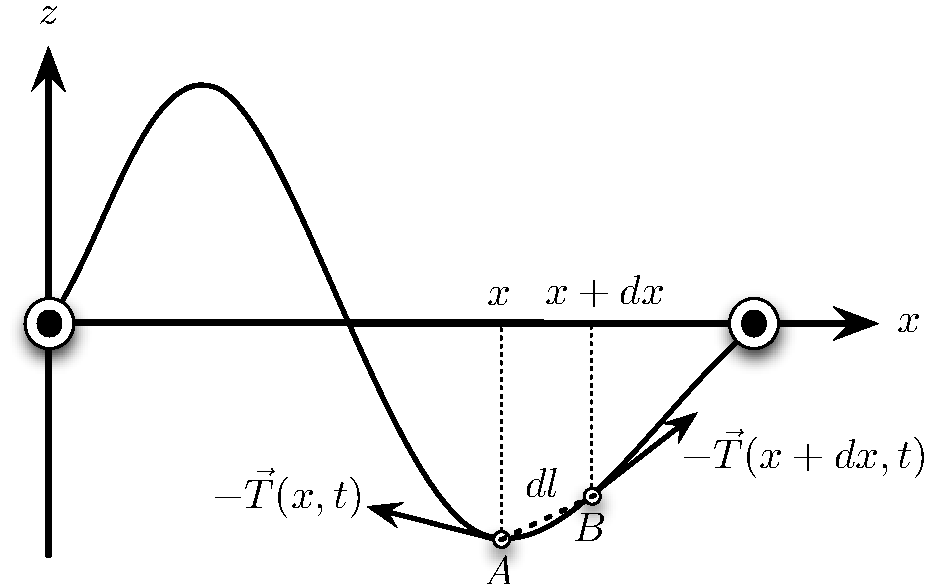
\includegraphics[width=0.6\textwidth]{Appendices/A/Pics/Pdf/DAlembert.pdf}
	\end{center}
	\vspace{-0.5cm}
	\caption[d'Alembert formulation of the vibrating string]{d'Alembert formulation of the vibrating string.}
	\label{fig:dalembert}
\end{figure}

The d'Alembert equation make two major assumptions:

\begin{itemize}
	\item The displacement of the string is mostly vertical and negligeable compared to the longitudinal displacement, \emph{i.e.} $z \ll x$ and consequently $\frac{\partial{z}}{\partial{x}} \ll 1$
	\item The gravity force applied on the string is negligeable
\end{itemize}

With these assumptions, the infinitesimal length $dl$ between $A$ and $B$ is such that:

$$
	dl^2 = dx^2 + [z(x+dx, t) - z(x, t)]^2 = dx^2 . [1 + (\frac{\partial{z}}{\partial{x}})^2] \sim_{z \ll x} dx^2
$$

Applying Newton's principle on the infinitesimal string length $dl$ leads to the system:

\begin{eqnarray}
	T_x(x+dx, t) - T_x(x, t) = 0  \label{eq:dalembert1} \\
   	T_z(x+dx, t) - T_z(x, t) = \mu . dx . \frac{\partial^2{z}}{\partial{t^2}}(x, t) \label{eq:dalembert2}
\end{eqnarray}

\myequname \eqref{eq:dalembert1} expresses the independance and constance of the longitudinal component of $T$ towards the longitudinal displacement $x$ and time $t$, so that we can deduce from the boundary conditions: $\forall x$, $\forall t$ $T_x(x, t) = T$. The tangency of the tension induces also: $\frac{T_z}{T_x} = \frac{\partial z}{\partial x}(x, t)$, so that $T_z(x, t) = T . \frac{\partial z}{\partial x}(x, t)$.

The substitution of the latter expressions in \myequname \eqref{eq:dalembert2} leads to:

\begin{equation}
	T_z(x+dx, t) - T_z(x, t) = T . dx . \frac{\partial^2 z}{\partial x^2}(x, t) = \mu . dx . \frac{\partial^2{z}}{\partial{t^2}}(x, t)
	\label{eq:dalembert3}
\end{equation}

From \myequname \eqref{eq:dalembert3}, we deduce the d'Alembert formulation enounced in \myequname \eqref{eq:soundPhysicsPDE}.


	\section{d'Alembert Equation: Fourier's Solution}
	\label{sec:ssDerivation_dalembertFourier}

Fourier proposed a general solution to d'Alembert equation of the vibrating string problem. It involves a particular form of the solution as a stationnary wave, such that $z(x, t) = z_1(t).z_2(x)$.

The substitution of such solution form in \myequname \eqref{eq:soundPhysicsPDE} leads to:

\begin{equation}
	\frac{\ddot{z_2}}{z_2}(x) = \frac{1}{c^2} . \frac{\ddot{z_1}}{z_1}(t)\ with\ c^2 = \frac{T}{\mu}
	\label{eq:fourier1}
\end{equation}

Due to the dependancy of the two members of \myequname \eqref{eq:fourier1} to two separable variables (space and time), these terms are inevitably equal to a real constant $a$. From that observation we can deduce a general form of the function $z_1$ and $z_2$, with $k_i = \frac{i\pi}{L}$, and $\phi_i$ depending on initial conditions:

$$
\begin{array}{c}
   	\ddot{z_1}(t) = a . c^2 . z_1(t) \Rightarrow z_1(t) = a_1 . sin(k_i . c . t + \phi_i)  \label{eq:fourier2} \\
	\ddot{z_2}(x) = a . z_2(x) \Rightarrow z_2(x) = a_2 . sin(k_i . x) \label{eq:fourier3}
\end{array}
$$

The solution can then be written as a sum of \emph{normal modes} $z_i$ characterizing the allowed modes of deformation of the string:

$$
	z(x, t) = \sum_{i=1}^{\infty} z_i(x, t)\ with\ z_i(x, t) =  a_{i}^{'} . \sin(k_i . c .t + \phi_i) . \sin(k_i . x)
$$

These normal modes can also be rewritten as:

\begin{equation}
	z_i(x, t) = a_i . [ \cos(k_i.(c.t - x) + \phi_i) - \cos(k_i.(c.t + x) + \phi_i) ]
	\label{eq:fourier4}
\end{equation}

\myequname \eqref{eq:fourier4} shows the form of the solution intuited by d'Alembert, composed of two travelling waves in opposite longitudinal directions, \myequname \eqref{eq:soundPhysicsPDE2}.

\newpage\vfill


	\section{Modal Decomposition and d'Alembert Equation}
	\label{sec:ssDerivation:modalDecomposition}

We consider here the simplest modal decomposition of a vibrating string of length $L$ composed of $n$ identical masses ($m$) linked by identical springs ($k$), \myfigname \ref{fig:modalDecomposition}. This representation makes the assumption that every mass is spaced of a distance $h$, that is negligeable, \emph{i.e.} $h \ll 1$ for continuity purpose and for treating the string as a continuous material.

\begin{figure}[H]
	\begin{center}
		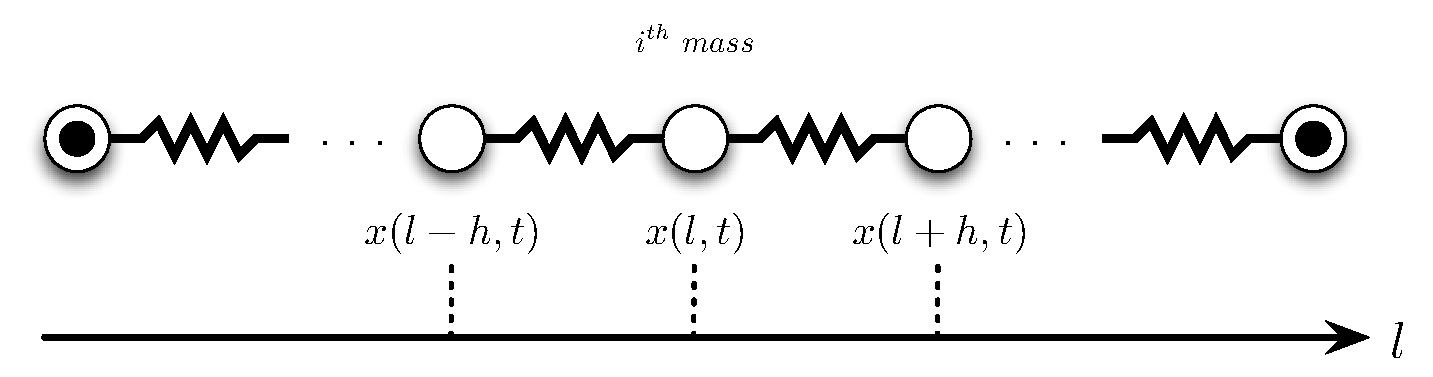
\includegraphics[width=0.8\textwidth]{Appendices/A/Pics/Pdf/ModalDecomposition.pdf}
	\end{center}
	\vspace{-0.5cm}
	\caption[Modal decomposition of the vibrating string]{Modal decomposition of the vibrating string.}
	\label{fig:modalDecomposition}
\end{figure}
	
Applying Newton's principle on the $i^{th}$ mass leads to the system, where the contributions of the previous and next masses are derived by the Hookes law:

\begin{eqnarray}
	m . \frac{\partial^2{x}}{\partial{l^2}}(l, t) = T_{l-h}(l, t) + T_{l+h}(l, t) \label{eq:modalDecomposition1} \\
	T_{l-h}(l, t) = -k . [x(l, t) - x(l-h, t)] \nonumber \\
	T_{l+h}(l, t) = k . [x(l+h, t) - x(l, t)] \nonumber
\end{eqnarray}

The continuity assumption allows the derivation of the following Taylor limited developments:

$$
\begin{array}{l}
	x(l-h, t) \sim_{h \ll 1} x(l, t) - h . \frac{\partial x}{\partial l} + \frac{h^2}{2} . \frac{\partial^2 x}{\partial l^2} \\
	x(l+h, t) \sim_{h \ll 1} x(l, t) + h . \frac{\partial x}{\partial l} + \frac{h^2}{2} . \frac{\partial^2 x}{\partial l^2}
\end{array}
$$

The substitution of the latter expressions into \myequname \eqref{eq:modalDecomposition1} leads finally to:

\begin{equation}
	\frac{\partial^2{x}}{\partial{l^2}}(l, t) - \frac{1}{c^2} . \frac{\partial^2{x}}{\partial{t^2}}(l, t) = 0\ with\ c^2 = \frac{k.h^2}{m} \label{eq:modalDecomposition2}
\end{equation}

Note that the dimension of the constant $c$ is the dimension of a velocity. Furthermore, the modal decomposition of the spring can be considered as whole spring by observing:

\begin{itemize}
	\item the mass of the system is equally distributed, such that we can consider a lineic mass $m_l = \frac{m}{h}$
	\item each spring is characterized by a constant stiffness $k$ at its steady distance $h$. Knowing that the stiffness of a spring is inversely proportional to its steady distance, we can express the stiffness of the whole spring as $k = \frac{k_l}{h}$ where $k_l$ is a charactertistic of the equivalent spring (note however that the dimension of $k_l$ is the dimension of a force [N] and not a stiffness).
\end{itemize}

We can eventually write the equation \myequname \eqref{eq:modalDecomposition2} that governs the motion of the string as follows:

\begin{equation}
	\frac{\partial^2{x}}{\partial{l^2}}(l, t) - \frac{1}{c^2} . \frac{\partial^2{x}}{\partial{t^2}}(l, t) = 0\ with\ c^2 = \frac{k_l}{m_l} \label{eq:modalDecomposition3}
\end{equation}

\myequname \eqref{eq:modalDecomposition3} is analogously to \myequname \eqref{eq:soundPhysicsPDE} of the form of the d'Alembert equation, justifying the use of such mechanical model for the problem of the vibration string.

\newpage\vfill


	\section{Finite-Difference and Finite-Element Formulations}
	\label{sec:ssDerivation:finiteDifferenceElement}

\noindent{\textbf{Finite-Difference}\\

The finite-difference formulation proceed to a discretization of \myequname \eqref{eq:soundPhysicsPDE} both in space and time. Given a fixed space step $\delta x$ such that $L = X_s\delta x$, and a fixed time step $\delta t$ such that $T = T_s\delta t$, a second order and explicit scheme leads to the following Taylor limited development of the partial derivatives:

$$
\begin{array}{c}
	\frac{\delta x^2}{2} . \frac{\partial^2 z}{\partial x^2} \sim_{\delta x \ll 1}  z(x-\delta x, t) - z(x, t) + \delta x . \frac{\partial z}{\partial x} \\
	\\
	\frac{\delta x^2}{2} . \frac{\partial^2 z}{\partial x^2} \sim_{\delta x \ll 1}  z(x+\delta x, t) - z(x, t) - \delta x . \frac{\partial z}{\partial x} \\
	\\
	\frac{\delta t^2}{2} . \frac{\partial^2 z}{\partial t^2} \sim_{\delta t \ll 1}  z(z, t-\delta t) - z(x, t) + \delta t . \frac{\partial z}{\partial t} \\
	\\
	\frac{\delta t^2}{2} . \frac{\partial^2 z}{\partial t^2} \sim_{\delta t \ll 1}  z(z, t+\delta t) - z(x, t) - \delta t . \frac{\partial z}{\partial t}
\end{array}
$$

Note that a continuity assumption is again made on the function $z$ for writing these Taylor series; the partial derivatives involved in the d'Alembert equation can also been expressed such that:

$$
\begin{array}{c}
	\frac{\partial^2 z}{\partial x^2} \sim_{\delta x \ll 1}  \frac{z(x+\delta x, t) - 2.z(x, t) + z(x-\delta x, t)}{\delta x^2} \\
	\\
	\frac{\partial^2 z}{\partial t^2} \sim_{\delta t \ll 1}  \frac{z(x, t+\delta t) - 2.z(x, t) + z(x. t-\delta t)}{\delta t^2}
\end{array}
$$

Solving the discretized problem is then equivalent to:

\begin{eqnarray}
	\forall t \in [1, T_s-1],\ \forall x \in [1, X_s-1] \nonumber \\
	\nonumber \\
	\frac{z[(x+1).\delta x, t] - 2.z[x, t] + z[(x-1).\delta x, t]}{\delta x^2} \nonumber \\
	- \frac{1}{c^2} . \frac{z[x, (t+1).\delta t] - 2.z[x, t] + z[x, (t-1).\delta t)}{\delta t^2}  = 0 \label{eq:FD}\\
	\nonumber
\end{eqnarray}

\noindent{\textbf{Finite-Element}\\

The finite-element method offers a more formalized formulation of the problem. The vertical displacement function $z$ of the string is first admitted to belong to the vectorial space $H_{[0, L]}$, composed of the functions whose square and square derivative can be integrated on $[0, L]$. The definition of a scalar product $< , >$ on $H_{[0, L]}$ is therefore possible: 

$$
	(f, g) \in H_{[0, L]} \times H_{[0, L]}\ <f, g>\ =\ \int_{0}^{L} f(x) . g(x) . dx
$$

This ensure that the integral $\int_{0}^{L} f(x)^2 . dx$ exists. Note that $H_{[0, L]}$ is also more constrained when taking into account the limit conditions imposed by the vibrating string problem, such that every function $f$ belonging to $H_{[0, L]}$ respect the following conditions: $f(0) = f(L) = 0$ and $\frac{\partial f}{\partial x}(0, 0) = \frac{\partial f}{\partial x}(L, 0) = T$, with $T$ the tension applied on the string.\\

Back to the vibrating string problem, the finite-element method expresses the equation of d'Alembert \myequname \eqref{eq:soundPhysicsPDE} as a variational formulation which corresponds to the virtual work principle. The problem is to find the function $z$ satisfying:

\begin{equation}
	\forall v \in H_{[0, L]}\ <\frac{\partial^2 z}{\partial x^2}, v> -\ \frac{1}{c^2} . <\frac{\partial^2 z}{\partial t^2}, v>\ =\ 0 
	\label{eq:finiteElement1}
\end{equation}

An integration by parts combined with the initial conditions leads to the following simplification:

$$
	<\frac{\partial^2 z}{\partial x^2}, v>\ =\ [\frac{\partial z}{\partial x} . v]_{0}^{L}\ - <\frac{\partial z}{\partial x}, \frac{\partial v}{\partial x}>\ =\ -<\frac{\partial z}{\partial x}, \frac{\partial v}{\partial x}>
$$

So that \myequname \eqref{eq:finiteElement1} is equivalent to finding $z$ satisfying:

\begin{equation}
	\forall v \in H_{[0, L]}\ <\frac{\partial z}{\partial x}, \frac{\partial v}{\partial x}> +\ \frac{1}{c^2} . <\frac{\partial^2 z}{\partial t^2}, v>\ =\ 0 
	\label{eq:finiteElement2}
\end{equation}

The discretization of \myequname \eqref{eq:finiteElement2} is achieved by approximating the problem on a finite vectorial subspace of $H_{[0, L]}$. For simplicity matters, we will consider the vectorial subspace $V_h$ of $H_{[0, L]}$ of dimension $N$ composed of the piecewise continuous functions with the following basis:

$$
	\forall i \in [1, N],\ \forall j \in [1, N]\ w_i(x_j) = \delta_{ij}  \nonumber
$$

It leads to the expression of any function $v_h$ belonging to $V_h$, with its geometric correspondance given in \myfigname \ref{fig:finiteElement1} (note that the equivalent discretization of the string can be not equally distributed).

\begin{equation}
	\forall v_h \in V_h\ v_h(x) = \sum_{i=1}^{n} v_i . w_i(x)\ with\ v_i = v_h(x_i) \label{eq:finiteElement3}
\end{equation}

\begin{figure}[H]
	\begin{center}
		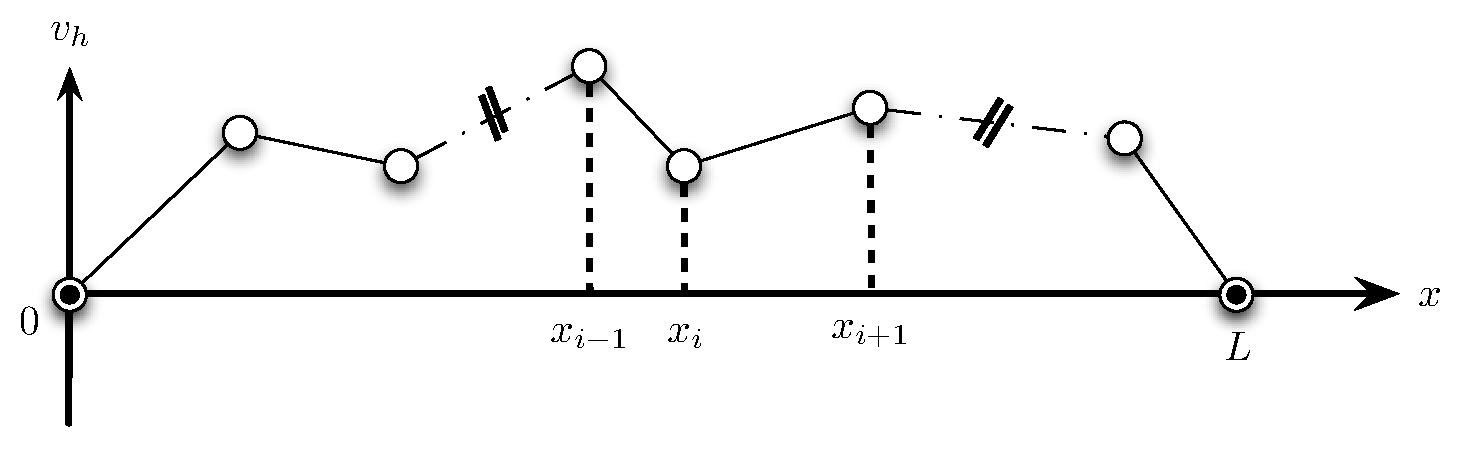
\includegraphics[width=\textwidth]{Appendices/A/Pics/Pdf/FiniteElement1.pdf}
	\end{center}
	\vspace{-0.5cm}
	\caption[Finite-element decomposition of the vibrating string]{Finite-element decomposition of the vibrating string.}
	\label{fig:finiteElement1}
\end{figure}

The function $z$ is analogously approximated in the subspace $V_h$ by a function $z_h$, and leads to the discretized problem of finding $z_h$ satisfying:

\begin{eqnarray}
	z_h(x, t) = \sum_{i=1}^{n} z_i(t) . w_i(x) \label{eq:finiteElement4} \\
	\forall v_h \in V_h\ <\frac{\partial z_h}{\partial x}, \frac{\partial v_h}{\partial x}> +\ \frac{1}{c^2} . <\frac{\partial^2 z_h}{\partial t^2}, v_h>\ =\ 0 \label{eq:finiteElement5}
\end{eqnarray}

By introducing the derivative forms of $v_h$ and $z_h$, \myequname \eqref{eq:finiteElement3} and \eqref{eq:finiteElement4}, into the discretized formulation, \myequname \eqref{eq:finiteElement5}, the final formulation of the finite-element model of the vibrating string is:

$$
\begin{array}{r}
	\forall t \in [0, T],\ \forall j \in [1, N],\ find\ z_j(t)\ so\ that \\
	\nonumber \\
	\forall i \in [1, N]\ \sum_{j=1}^{n} (\int_{0}^{L}\frac{\partial w_j}{\partial x} . \frac{\partial w_i}{\partial x} . dx) . z_j(t) + \frac{1}{c^2} . \sum_{j=1}^{n} (\int_{0}^{L} w_j . w_i . dx) . \frac{\partial^2 z_j}{\partial t^2}(t) = 0  
\end{array}
$$

This can also be written in a matrical form:

\begin{eqnarray}
	\forall t \in [0, T],\ find\ \boldsymbol{Z}(t)\ so\ that \nonumber \\
	\nonumber \\
	\boldsymbol{M} . \ddot{\boldsymbol{Z}}(t) + \boldsymbol{K} . \boldsymbol{Z}(t) = 0 \label{eq:finiteElement6} \\
	\nonumber \\
	\boldsymbol{Z}(t) = [z_j(t)]_{j \in [1, N]} \nonumber \\
	\boldsymbol{M} = [m_{ij}]_{(i, j) \in [1, N]\times[1, N]}\ with\ m_{ij} = \frac{1}{c^2} . \int_{0}^{L} w_j . w_i . dx \nonumber \\
	\boldsymbol{K} = [k_{ij}]_{(i, j) \in [1, N]\times[1, N]}\ with\ k_{ij} = \int_{0}^{L}\frac{\partial w_j}{\partial x} . \frac{\partial w_i}{\partial x} . dx \nonumber
\end{eqnarray}

The matrices $\boldsymbol{M}$ and $\boldsymbol{K}$ are called respectively the mass and stiffness matrices of the system. In our case, $V_h$ is the vectorial subspace composed of the piecewise continuous functions, so that $\boldsymbol{M}$ and $\boldsymbol{K}$ can be easily expressed knowing the line equation of each basis function $w_i$.\\

\myequname \eqref{eq:finiteElement6} can then be discretized in time according to a similar scheme described in the previous point regarding the finite-difference formulation. By defining a time step $\delta t$ such that $T = T_s\delta t$, an explicit scheme of the second order leads to solving:

\begin{eqnarray}
	\forall t \in [1, T_s-1],\ find\ \boldsymbol{Z}[(t+1).\delta t]\ so\ that \nonumber \\
	\nonumber \\
	\boldsymbol{M} . \boldsymbol{Z}[(t+1).\delta t] = (2\boldsymbol{M} + \delta t^2 . \boldsymbol{K}) . \boldsymbol{Z}[t . \delta t] + \boldsymbol{M} . \boldsymbol{Z}[(t-1).\delta t]
\end{eqnarray}

\newpage\vfill


	\section{Digital Waveguide Formulation}
	\label{sec:ssDerivation:dW}

\noindent{\textbf{Karplus-Strong}\\

\myfigname \ref{fig:kP} and \myequname \eqref{eq:kP} describe the formulation of Karplus and Strong for synthesizing sounds from a delay line of length $p$ for the vibrating string problem. The delay line is initialized randomly by numbers, and the synthesis is achieved by a given modifier that acts on the delay line. The modifier in the case of the vibrating string can be considered as a low-pass filter that accounts for the decay of the tone.

\begin{equation}
	z(n) = \frac{1}{2} . [z(n - p) + z(n - p - 1)] \label{eq:kP}
\end{equation}

\begin{figure}[H]
	\begin{center}
		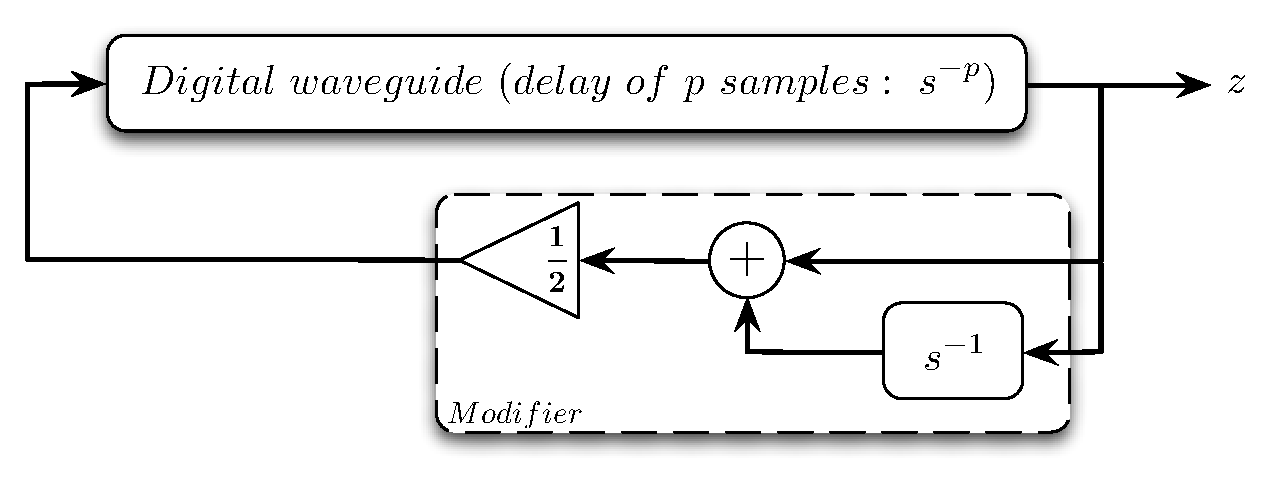
\includegraphics[width=0.8\textwidth]{Appendices/A/Pics/Pdf/KP.pdf}
	\end{center}
	\vspace{-0.5cm}
	\caption[Karplus-Strong delay line of the vibrating string]{Karplus-Strong delay line of the vibrating string.}
	\label{fig:kP}
\end{figure}

The method of Karplus and Strong is a somewhat \emph{ad-hoc} formulation of the vibrating string problem since it introduces the design of a filter.\\

\noindent{\textbf{Digital Waveguide and Finite-Difference Scheme Equivalence}\\

\myfigname \ref{fig:Smith} depicts the two delay lines involved in the digital waveguide formulation of the vibrating string problem.

\begin{figure}[H]
	\begin{center}
		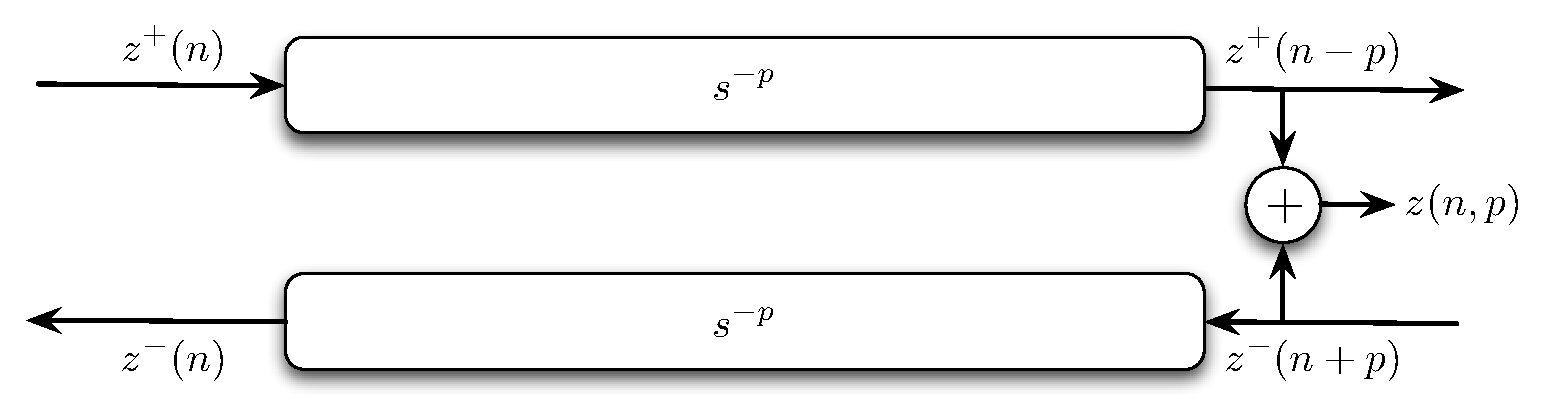
\includegraphics[width=0.95\textwidth]{Appendices/A/Pics/Pdf/Smith.pdf}
	\end{center}
	\vspace{-0.5cm}
	\caption[Digital waveguide delay lines of the vibrating string]{Digital waveguide delay lines of the vibrating string}
	\label{fig:Smith}
\end{figure}

The physical interpretation of the digital waveguide formulation can be obtained from the equivalence to the finite-difference method. By normalizing the simulation terms $\delta x$, $\delta t$ and $c$, \myequname \eqref{eq:FD} becomes:

\begin{equation}
	z(n+1, p) = z(n, p+1) - z(n-1, p) + z(n, p-1) \label{eq:dW1}
\end{equation}

As stated by the digital waveguide formulation $z(n, p) = z^{+}(n-p) + z^{-}(n+p)$, so that:


\begin{eqnarray}
	z(n, p+1) - z(n-1, p) + z(n, p-1) & = & z^{+}(n-p-1) + z^{-}(n+p+1) \nonumber \\
	& & - z^{+}(n-1-p) - z^{-}(n-1+p) \nonumber \\
	& & + z^{+}(n-p+1) + z^{-}(n+p-1) \nonumber \\
	& = & z^{+}(n-p+1) + z^{-}(n+p+1) \nonumber \\
	& = & z^{+}[(n+1)-p] + z^{-}[(n+1)+p] \nonumber \\
	& = & z(n+1, p) \label{eq:dW2}
\end{eqnarray}

\myequname \eqref{eq:dW1} and \eqref{eq:dW2} are then proved to be equivalent. Moreover \myequname \eqref{eq:dW2} can be expressed such that:

\begin{eqnarray}
	z(n+1, p) & = & z^{+}[(n+1)-p] + z^{-}[(n+1)+p] \nonumber \\
	& = & z^{+}[n - (p-1)] + z^{-}[n + (p+1)] \label{eq:dW3}
\end{eqnarray}

\myequname \eqref{eq:dW3} expresses the vertical displacement of the string at the position $p$ at the time $n+1$ as the superposition of the left-going and right-going string displacements at the time $n$ at the positions $p-1$ and $p+1$, which is exactly the scheme depicted by \myfigname \ref{fig:Smith}.

\newpage\vfill


	\section{Modal Synthesis Formulation}
	\label{sec:ssDerivation:mM}

\noindent{\textbf{Normal Shapes and Modes}\\

Let us recall \myequname \eqref{eq:soundPhysicsMM}, governing the motion of $N$ coupled oscillators:

\begin{equation}
	\boldsymbol{M} . \ddot{\boldsymbol{z}}(t) + \boldsymbol{K} . \boldsymbol{z}(t) = 0 \label{eq:mM1}
\end{equation}

We look for a factorized solution of the oscillation form $\boldsymbol{z}(t) = \boldsymbol{s} . \sin(\omega.t + \phi)$, $\boldsymbol{s}$ are called the \emph{modal shapes} of the system, so that the previous equation becomes:

\begin{equation}
	\boldsymbol{\omega}^2 . \boldsymbol{M} . \boldsymbol{s} = \boldsymbol{K} . \boldsymbol{s} \Leftrightarrow \ \boldsymbol{M}^{-1} . \boldsymbol{K} . s = \boldsymbol{\omega}^2 . \boldsymbol{s} \label{eq:mM2}
\end{equation}

The system described by \myequname \eqref{eq:mM2} is then characterized by $N$ eigenvalues $\boldsymbol{\omega}^2$ and eigenvectors $\boldsymbol{s}$ (the \emph{modal shapes}) of the matrix $\boldsymbol{M}^{-1} . \boldsymbol{K}$. The \emph{modal shapes} form then an orthogonal basis of the system, such that:

$$
\begin{array}{c}
	\forall (i, j) \in [1, N]\times[1, N] \\
	s_j^T . \boldsymbol{M} . s_i = \delta_{ij} . m_i \\
	s_j^T . \boldsymbol{K} . s_i = \delta_{ij} . k_i\ with\ k_i = \omega_i^2 . m_i
\end{array}
$$

The \emph{modal shapes} define therefore a coordinate \emph{modal transformation} from a system of $N$ coupled oscillators to a system of $N$ \emph{uncoupled} normal modes noted $\boldsymbol{q}$, such that:

\begin{equation}
	\boldsymbol{z} = \boldsymbol{S} . \boldsymbol{q} \Leftrightarrow \ \boldsymbol{q} = \boldsymbol{S}^T . \boldsymbol{z} \label{eq:mM3}
\end{equation}

Solving \myequname \eqref{eq:mM1} is then equivalent to solve the system described by \myequname \eqref{eq:mM4}:

\begin{eqnarray}
	\boldsymbol{M}_S . \ddot{\boldsymbol{q}}(t) + \boldsymbol{K}_S . \boldsymbol{q}(t) = 0 \label{eq:mM4} \\
	with\ \boldsymbol{M}_S = \boldsymbol{S}^T . \boldsymbol{M} . \boldsymbol{S}\ and\ \boldsymbol{K}_S = \boldsymbol{S}^T . \boldsymbol{K} . \boldsymbol{S} \nonumber
\end{eqnarray}

$\boldsymbol{M}_S$ and $\boldsymbol{K}_S$ are diagonal mass and stiffness matrices by the transformation $\boldsymbol{S}$. Once the system described by \myequname \eqref{eq:mM4} is solved, $\boldsymbol{z}$ is then obtained through a linear combination of the \emph{normal modes} $\boldsymbol{q}$ weighted by the \emph{modal shapes}, accordingly to \myequname \eqref{eq:mM3}:

$$
	\forall j \in [1, N]\ z_j(t) = \sum_{i = 0}^{N} s_{i, j} . q_i(t) \\
$$

\newpage

\noindent{\textbf{Continuous Equivalence}\\

Back to the vibrating string problem, let us recall the d'Alembert equation \myequname \eqref{eq:soundPhysicsPDE}: 

$$
	T.\frac{\partial^2{z}}{\partial{x^2}}(x, t) - \mu.\frac{\partial^2{z}}{\partial{t^2}}(x, t) = 0
$$

From section \ref{sec:ssDerivation_dalembertFourier}, we already know that $z$ is of the form $z(x, t) = \sum_{i=1}^{N} z_i(x, t)$ with $z_i(x, t) = s_i(x).q_i(t)$. By introducing this latter expression in \myequname \eqref{eq:soundPhysicsPDE}, multiplying by $s_i$ and integrating over the string length leads to:

\begin{equation}
	\forall i \in [1, N]\ [\mu . \int_{0}^{L} s_i^2(x) . dx] . \frac{d^2 q_i}{dt^2}(t) - [T . \int_{0}^{L} \frac{d^2 s_i}{dx^2}(x) . s_i(x) . dx] . q_i(t) = 0 \label{eq:mM5}
\end{equation}

An integration by parts combined with the initial conditions leads to the following simplification:

$$
	\forall i \in [1, N]\ \int_{0}^{L} \frac{d^2 s_i}{dx^2}(x) . s_i(x) . dx = [\frac{d s_i}{dx}(x) . s_i(x)]_{0}^{L}\ - \int_{0}^{L} [\frac{d s_i}{dx}(x)]^2 . dx = - \int_{0}^{L} [\frac{d s_i}{dx}(x)]^2 . dx
$$

\myequname \eqref{eq:mM5} becomes therefore:

$$
	\forall i \in [1, N]\ [\mu . \int_{0}^{L} s_i^2(x) . dx] . \frac{d^2 q_i}{dt^2}(t) + [T . \int_{0}^{L} [\frac{d s_i}{dx}(x)]^2 . dx] . q_i(t) = 0
$$

This latter expression can also be expressed as a matricial equation, \myequname \eqref{eq:mM6} is then exactly of the form of \myequname \eqref{eq:mM1}

\begin{eqnarray}
	\boldsymbol{M} . \ddot{\boldsymbol{q}}(t) + \boldsymbol{K} . \boldsymbol{q}(t) = 0 \label{eq:mM6} \\
	\boldsymbol{M} = [m_i]_{i \in [1, N]}\ with\ m_i = \mu . \int_{0}^{L} s_i^2(x) . dx \nonumber \\
	\boldsymbol{K} = [k_i]_{i \in [1, N]}\ with\ k_i = T . \int_{0}^{L} [\frac{d s_i}{dx}(x)]^2 . dx \nonumber
\end{eqnarray}






